\documentclass[]{book}
\usepackage{import}
\usepackage{preamble}
\usepackage{tikz}

\begin{document}

\noindent BECA / Huson / 11.1 IB Math SL \hspace{2in} Name:\\*
6 November 2017
\begin{center}
{\Large Review: Exponents and radicals (easier)}\\
\textit{Do these problems without a calculator. Use algebra properties to simplify each expression.}
\end{center}

%\vspace{0.2 cm}
\begin{enumerate}

\subsection*{Exponent rules}

\item $\displaystyle 4x^{2} \times x^4 y^3$\\[10pt]
\item $a^3 b \div a^{2}$\\[10pt]
\item $(x^2 y^2)^2 \times (x^3 y)$\\[10pt]
\item $\displaystyle (\frac{1}{2} x^3)^2$\\[10pt]

\subsection*{Fractional and negative exponents}
Simplify. Express as fractions or radicals

\item $\displaystyle  49^\frac{1}{2}$\\[10pt]
\item $\displaystyle  (xy)^\frac{1}{2}$\\[10pt]
\item $\displaystyle  (ab)^{-1}$\\[10pt]
\item $\displaystyle  (x^2 y)^{-2}$\\[10pt]

\subsection*{Radicals and exponents}
Simplify, leaving no negative or fractional exponents.

\item $\sqrt{x^4 y^2}$\\[10pt]
\item $\displaystyle  \frac{\sqrt[3]{8x}}{4}$\\[10pt]
\item $\displaystyle  \sqrt{\frac{x^2 y^{6}}{z^{4}}}$\\[10pt]
\end{enumerate}

\newpage 

\noindent BECA / Huson / 11.1 IB Math SL \hspace{2in} Name:\\*
6 November 2017
\begin{center}
{\Large Review: Exponents and radicals (challenge)}\\*
\textit{Do these problems without a calculator. Answer the first page on loose leaf paper.}
\end{center}

%\vspace{0.2 cm}
Simplify, leaving no negative or fractional exponents.

\begin{enumerate}

\item $\displaystyle \frac{3}{4} a^{-3} \times a^3 b^{-3}$ \\*[5pt]
    %$\displaystyle =\frac{2x^2}{9y^3}$\\*[10pt]
\item $\displaystyle  \frac{2 \sqrt{36x^2}}{\sqrt[3]{27x^{3}}}$\\*[5pt]
    %$\displaystyle =\frac{5x^5}{\sqrt[3]{7}}$\\[10pt]
\item $x^3 y^{-2} \times (\frac{x}{y^2})^{-1}$
    %$\displaystyle =\frac{x^7}{y^5}$\\[10pt]
\item $(-2x^2 y)^2$
    %$=a^4$

\item $\displaystyle \frac{2}{3} (x^{-2} y)^3 \times \frac{6}{11}(x^2 y^{-1})$
    %$\displaystyle =\frac{2}{5}y$\\[10pt]
\item $\displaystyle  49^\frac{1}{4}$\\*[5pt]
    %$= \sqrt{7}$
\item $\displaystyle  \sqrt[3]{\frac{a^3 b^{-9}}{z^{-6}}}$\\*[5pt]
    %$\displaystyle = \frac{x^2 z}{y^4}$\\[10pt]

\item Let $f(x) = x^2 -6x - 7$.
\begin{enumerate}
    \item Show that the roots of $f(x)$ are 7 and $-1$.
    \item Rewrite $f(x)$ in vertex form. (complete the square) %$f(x)=(x-0)^2-4$. 
    \item Hence, state the vertex as an ordered pair.
        %Vertex: $(0,-4)$
    \item The function $g(x)$ is made by translating $f(x)$ right two units and up one unit. Write down the vertex of $g(x)$.
        %$g(x)=(x+5)^2-2$.
        \item Find the $y$-intercept of $g(x)$.
    \item Find the zeros of $g(x)$.
        %Translate left five units and up two units.
\end{enumerate}

\item Let $f(x) = (x-3)^2 - 4x$ and $g(x)=2x-5$. 
\begin{enumerate}
    \item Find $g^{-1}(x)$
    \item Find $(f \circ g) (x)$
    %$f(g(x))=((3x-2)-2)^2-3(3x-2)=9x^2-33x+22$
\end{enumerate}

\item Let $f(x) = 2x^2 +kx + 2$.
\begin{enumerate}
    \item $f(x)$ has exactly one root. Find $k$.
    \item $g(x)=-f(x)+4$. Find the solution(s) to $g(x)=f(x)$
\end{enumerate}
    
\item Let $f(x) = x^2+3x-1$ and $g(x)=2x-3$. Find $(f \times g)(x)$

\newpage 

\item Let $ f(x) = \frac{1}{3}(3)^x$, for $-3 \leq x \leq 3$.
\begin{enumerate}
\item On the  grid below, graph $f$.
\item Write down the value of $f(0)$.\\*
    %$f(0)=1$
\item Using the graph, solve for $f(x)= 1$.\\*
    %$f(2)= \frac{1}{4}$, therefore $x=2$
\item What is the value of $f^{-1}(9)$?\\*
    %$f^{-1}(8)=-3$
\end{enumerate}



\begin{figure}[!htbp]
\begin{center}
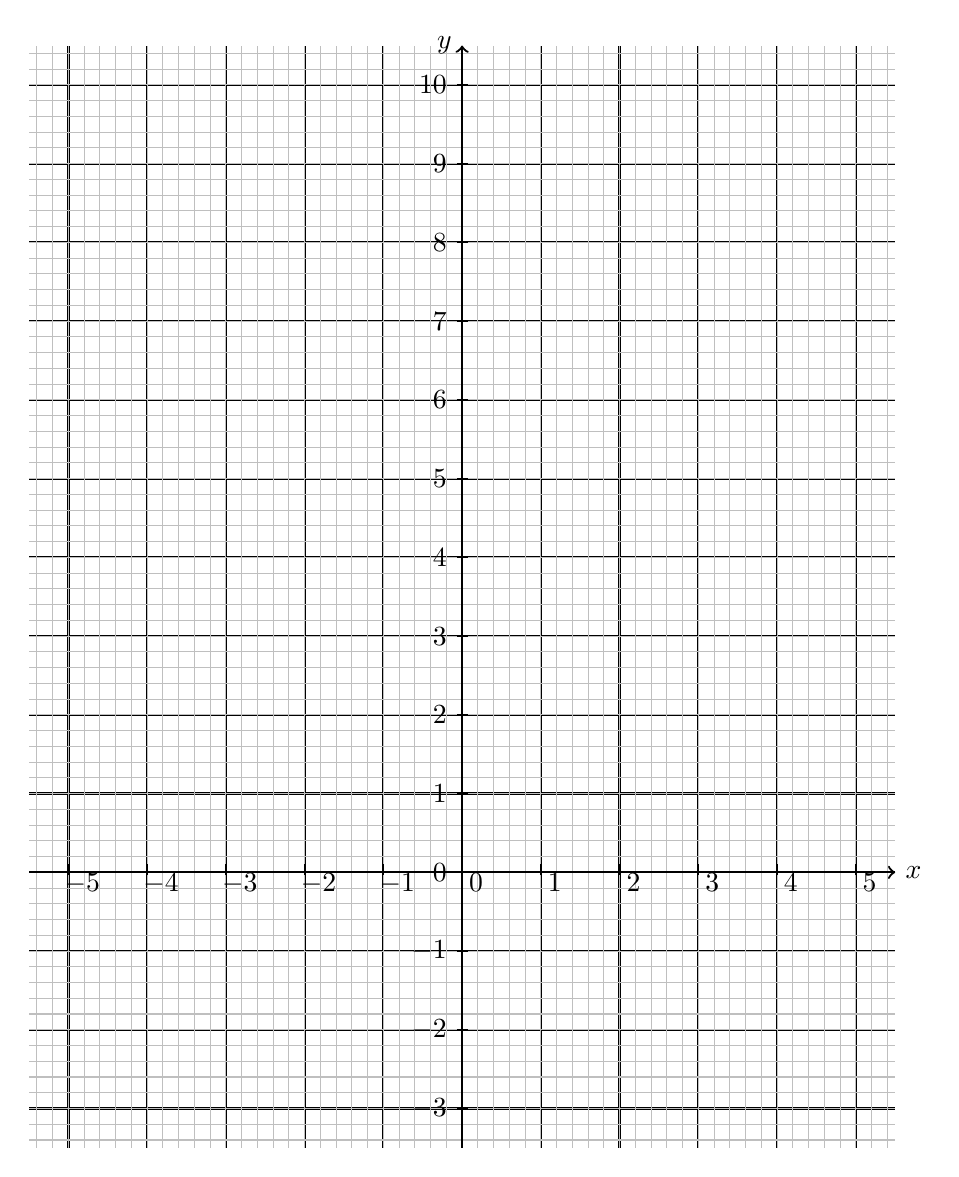
\begin{tikzpicture}

%grid
\draw [thick, color=black,, xstep=1.0cm,ystep=1.0cm] (-5.5,-3.5) grid (5.5,10.5);
\draw [thin, color=lightgray,, xstep=0.2cm,ystep=0.2cm] (-5.5,-3.5) grid (5.5,10.5);

\foreach \x in {-5, -4, -3, -2, -1, 0,1,2,3,4,5}
\draw[shift={(\x,0)},color=black] (0pt,-1pt) -- (0pt,3pt) node[below]  {$\quad \x$};

\foreach \y in {-3, -2, -1, 0,1,2,3,4,5, 6, 7, 8, 9, 10}
\draw[shift={(0,\y)},color=black] (2pt,0pt) -- (-2pt,0pt) node[left]  {$\y$};

\draw [thick, ->] (-5.5,0) -- (+5.5,0) node [right] {$x$};
\draw [thick, ->] (0,-3.5) -- (0,10.5) node [left] {$y$};

%\draw [-, -] plot[domain= -4:3] (\x, {1/3 * 3^\x}); %solution

\end{tikzpicture}
\end{center}
\end{figure}

\newpage 

\item The function $f(x)=e^x$ is shown on the graph. Sketch $g(x)=f(x)+1$. Plot and label the asymptote.

\begin{figure}[!htbp]
\begin{center}
\begin{tikzpicture}

%grid
%\draw [thick, color=black,, xstep=1.0cm,ystep=1.0cm] (-5.5,-1.5) grid (5.5,16.5);
%\draw [thin, color=lightgray,, xstep=0.2cm,ystep=0.2cm] (-5.5,-1.5) grid (5.5,16.5);

\foreach \x in {-5, -4, -3, -2, -1, 0,1,2,3,4,5}
\draw[shift={(\x,0)},color=black] (0pt,-3pt) -- (0pt,3pt) node[below]  {$\x$};

\foreach \y in {-1,0,1,2,3,4,5, 6, 7}
\draw[shift={(0,\y)},color=black] (2pt,0pt) -- (-2pt,0pt) node[left]  {$\y$};

\draw [thick, ->] (-5.5,0) -- (+5.5,0) node [right] {$x$};
\draw [thick, ->] (0,-1.0) -- (0,7.5) node [left] {$y$};

\draw [<->] plot[domain= -3:2] (\x, e^\x);
%\draw [dashed, <->] plot[domain= -1:5] (\x, {e^(\x-3)})  node[left]  {$g(x)$}; %Solution
 
\end{tikzpicture}
\end{center}
\end{figure}

\item The function $f(x)=e^x$ is shown on the graph. Sketch $g(x)=-f(x)+5$. Plot and label the asymptote.

\begin{figure}[!htbp]
\begin{center}
\begin{tikzpicture}

%grid
%\draw [thick, color=black,, xstep=1.0cm,ystep=1.0cm] (-5.5,-1.5) grid (5.5,16.5);
%\draw [thin, color=lightgray,, xstep=0.2cm,ystep=0.2cm] (-5.5,-1.5) grid (5.5,16.5);

\foreach \x in {-5, -4, -3, -2, -1, 0,1,2,3,4,5}
\draw[shift={(\x,0)},color=black] (0pt,-3pt) -- (0pt,3pt) node[below]  {$\x$};

\foreach \y in {-1,0,1,2,3,4,5, 6, 7}
\draw[shift={(0,\y)},color=black] (2pt,0pt) -- (-2pt,0pt) node[left]  {$\y$};

\draw [thick, ->] (-5.5,0) -- (+5.5,0) node [right] {$x$};
\draw [thick, ->] (0,-1.0) -- (0,7.5) node [left] {$y$};

\draw [<->] plot[domain= -3:2] (\x, e^\x);
%\draw [dashed, <->] plot[domain= -3:2] (\x, {-e^(\x)+5}) node[above]  {$g(x)$}; %Solution
%\draw [dotted, <->] plot[domain= -2.5:5] (\x, 5) node[below]  {$y=5$}; %Solution


\end{tikzpicture}
\end{center}
\end{figure}

\newpage
\item Graph the function $f(x) = 2^x$ on the grid below. 
\begin{enumerate}
    \item Label the $y$-intercept as an ordered pair.
    \item Label the point representing the solution to the equation $f(x)=4$ as an ordered pair.
    \item Write down the value of $f^{-1}(\frac{1}{2})$ and label the point on the graph of $f$.
        %$f^{-1}(-3)=1$
    \item Graph the inverse function, $f^{-1}(x)$.\\*
    Hint: plot the three points above, reversing the $x$ and $y$.
\end{enumerate}

\begin{figure}[!htbp]
\begin{center}
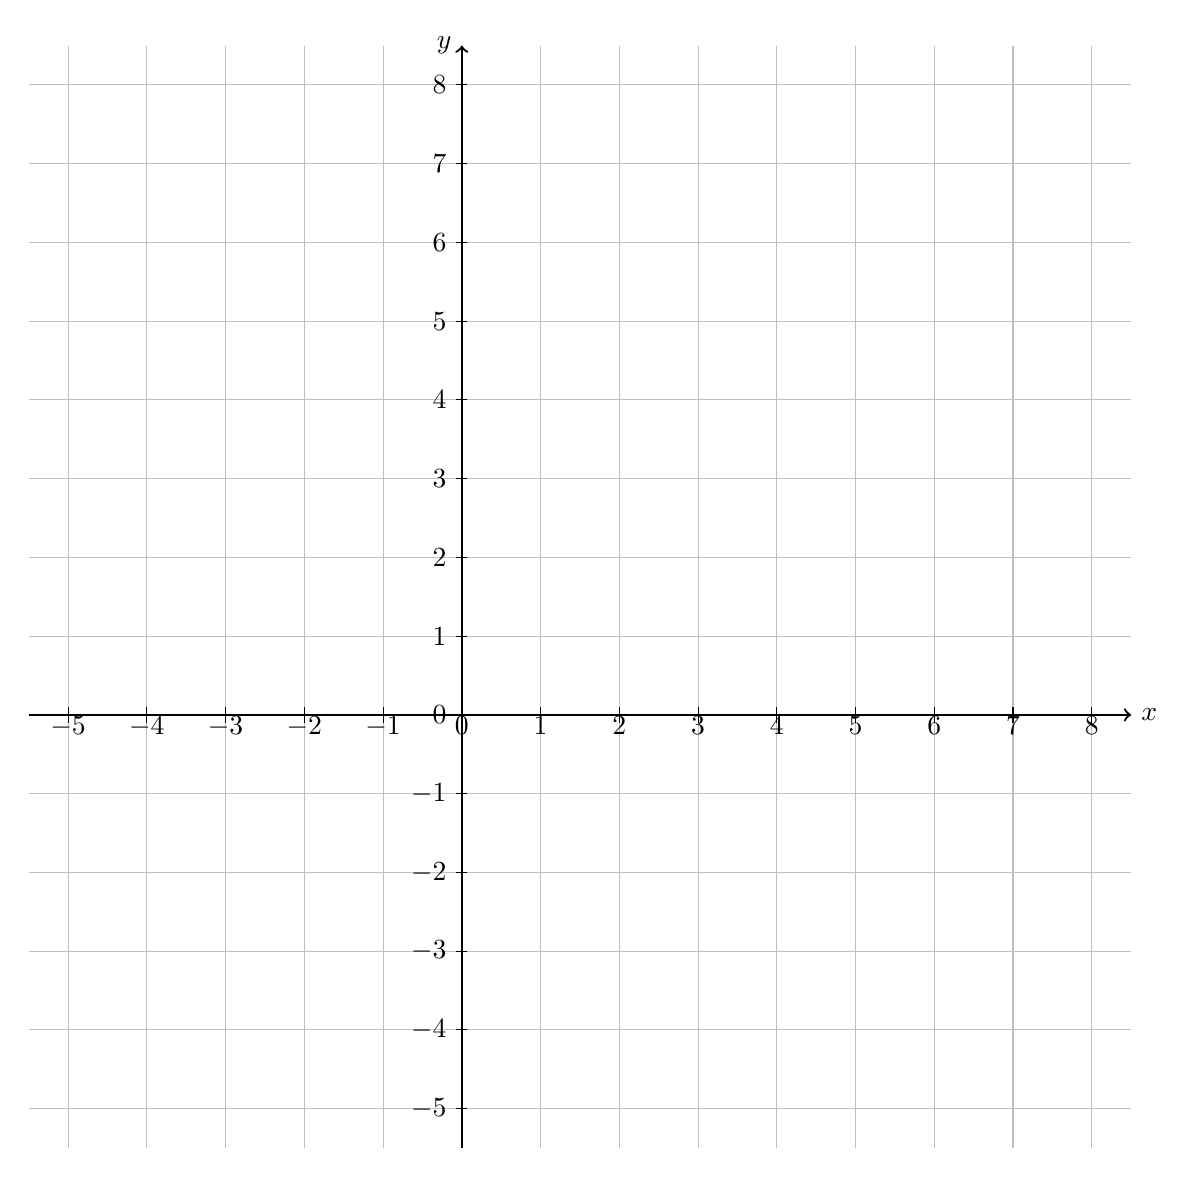
\begin{tikzpicture}

%grid
\draw [thin, color=lightgray,, xstep=1.0cm,ystep=1.0cm] (-5.5,-5.5) grid (8.5,8.5);
%\draw [thin, color=lightgray,, xstep=0.2cm,ystep=0.2cm] (-5.5,-1.5) grid (5.5,16.5);

\foreach \x in {-5, -4, -3, -2, -1, 0,1,2,3,4,5, 6, 7, 8}
\draw[shift={(\x,0)},color=black] (0pt,-3pt) -- (0pt,3pt) node[below]  {$\x$};

\foreach \y in {-5, -4, -3, -2, -1, 0,1,2,3,4,5, 6, 7, 8}
\draw[shift={(0,\y)},color=black] (2pt,0pt) -- (-2pt,0pt) node[left]  {$\y$};

\draw [thick, ->] (-5.5,0) -- (+8.5,0) node [right] {$x$};
\draw [thick, ->] (0,-5.5) -- (0,8.5) node [left] {$y$};

%\draw [->] plot[domain= -5:3] (\x, 2^\x) node[right] {$f(x)$}; %solution
%\draw [->] plot[domain= -5:3] (2^\x, \x) node[below] {$f^{-1}(x)$}; 

%\draw [fill] (0,1) circle (0.5ex) node[right] {$(a)\quad (0,1)$};
%\draw [fill] (2,4) circle (0.5ex) node[below] {$(b)\quad (2,4)$}; %solution
%\draw [fill] (-1,.5) circle (0.5ex) node[right] {$(c)\quad (-1,\frac{1}{2})$};

\end{tikzpicture}
\end{center}
\end{figure}



\end{enumerate}

\end{document}